\documentclass[10pt,aps,pra,twocolumn,superscriptaddress]{revtex4-1}

\usepackage{amsmath,amsthm}
\usepackage{amssymb}
\usepackage{amscd}
\usepackage{wasysym}
\usepackage[ansinew]{inputenc}
\usepackage[T1]{fontenc}
\usepackage{ae,aecompl}

   
    \usepackage[pdftex]{graphicx}
    \DeclareGraphicsExtensions{.pdf}

\usepackage{color}
\definecolor{red}{rgb}{1,0,0}
\definecolor{lred}{rgb}{1,0.7,0.7}
\definecolor{lgreen}{rgb}{0.7,1,0.7}

\usepackage{colortbl}



% -- new commands -------------------------------------------

\newtheorem{thm}{Theorem}
\newtheorem{defn}[thm]{Definition}

\newcommand{\abs}[1]{\vert#1\vert}
\newcommand{\be}{\begin{equation}}
\newcommand{\ee}{\end{equation}}
\newcommand{\bea}{\begin{eqnarray}}
\newcommand{\eea}{\end{eqnarray}}
\newcommand{\nn}{\nonumber}
\newcommand{\ket}[1]{|#1\rangle}
\newcommand{\bra}[1]{\left\langle#1\right|}
\newcommand{\braket}[2]{\langle{#1}|{#2}\rangle}
\newcommand{\eye}{\mbox{$\mbox{1}\!\mbox{l}\;$}}
\newcommand{\E}{{\cal E}}
\newcommand{\N}{{\cal N}}
\newcommand{\EE}{\mathbf{E}}
\newcommand{\PP}{\mathbf{P}}
\newcommand{\HH}{\mathcal{H}}
\newcommand{\tr}{{\rm tr}}
%\renewcommand{\vec}[1]{\mathbf{#1}}
\newcommand{\F}{{\cal F}}
\newcommand{\PR}{\mathcal{PR}}
\newtheorem{theorem}{Theorem}
\newtheorem{corr}{Corollary}
\newtheorem{claim}{Claim}
\newtheorem{problem}{Problem}



% --- front matter ---------------------------------------------

\begin{document}
\bibliographystyle{apsrev}
\title{Supplementary Information}

\author{Debsankha Manik}
\affiliation{Network Dynamics, Max Planck Institute for Dynamics and Self-Organization (MPIDS), Am Fassberg 17, D--37077 G\"ottingen, Germany}

\author{Benjamin Sch\"afer}
\affiliation{Network Dynamics, Max Planck Institute for Dynamics and Self-Organization (MPIDS), Am Fassberg 17, D--37077 G\"ottingen, Germany}

\author{Moritz Matthiae}
\affiliation{Network Dynamics, Max Planck Institute for Dynamics and Self-Organization (MPIDS), Am Fassberg 17, D--37077 G\"ottingen, Germany}


\author{Marc Timme}
\affiliation{Network Dynamics, Max Planck Institute for Dynamics and Self-Organization (MPIDS), Am Fassberg 17, D--37077 G\"ottingen, Germany}
\affiliation{Faculty of Physics, Georg August University G\"ottingen,
  Germany}

\author{Dirk Witthaut}
\affiliation{Network Dynamics, Max Planck Institute for Dynamics and Self-Organization (MPIDS), Am Fassberg 17, D--37077 G\"ottingen, Germany}

\date{\today }


%\begin{abstract}
%XXX
%\end{abstract}


\maketitle

% --- Content --------------------------------------------------------------------

\section{Introduction}

Don't spend time on the introduction yet. We'll write that later.

\section{An oscillator model for powergrid operation}

We model the power grid as a network of $N$ rotating synchronous machines 
\cite[p.~20]{Mach08}
representing, for instance, wind turbines, or electric motors \cite{Prab94,Fila08,12powergrid}. Each machine 
$j \in \{1,\ldots,N\}$
is characterized by the mechanical power $P^{\rm mech}_j$ it 
generates ($P^{\rm mech}_j > 0$) or consumes 
($P^{\rm mech}_j < 0$). The state of each rotating machine is 
determined by its mechanical phase angle $\phi_j(t)$ and 
its velocity $d \phi_j / dt$ and the dynamics is goverened 
by the \emph{swing equation}:
\be
\label{eq-swing}
   I_j \frac{d^2 \phi_j}{dt^2} + D_j \frac{d \phi_j}{dt}
    = P_j^{\rm mech} - P_j^{\rm el},
\ee
where $I_j$ is the machine's moment of inertia and $D_j$
is the damping torque coefficient.  The mechanical phase angle $\phi_j(t)$ 
equals the electric phase angle for a two-pole machine. Otherwise
both are related by a constant factor.
If a generator is decoupled from the grid in an uncontrolled way 
such that $P_j^{\rm el} = 0$, it accelerates until finally an 
emergency shutdown is performed.

%\subsection{Electrical power in AC circuits}
The electrical power in an AC circuit is:
\begin{equation}
\label{def-real-power}
\begin{aligned}
P(t)&=V(t)I(t)\\
&=V_{0}\cos{(\omega_0 t)}I_{0}\cos{(\omega_0 t+\delta)}\\
&=\frac{V_{0}I_{0}}{2}\left[\cos{\delta} + \cos{(2\omega_0 t+\delta)} \right]\\
&=\underbrace{V_{rms}I_{rms} \cos{\delta}}_{P_{real}} + V_{rms}I_{rms}\cos{(2\omega_0 t+\delta)}
\end{aligned}
\end{equation}

Out of this, the second term  adds up to zero when summed over a full period of 
the AC cycle. The first term constitutes 
the \emph{real power} flow from generator to consumers. It is convenient to 
adopt the complex notation at this point:

\begin{equation}
\label{}
\begin{aligned}
\tilde{V}&=V_{rms}e^{i\omega_0 t} &,\quad & \tilde{I}&=&I_{rms}e^{i(\omega_0 t+\delta)}\\
\tilde{P}&=\tilde{V}\tilde{I}^* &,\quad & P_{real}&=&Re(\tilde{P})
\end{aligned}
\end{equation}

Now we are in a position to calculate ${P_j^{el}}$ in \eqref{eq-swing}:
\begin{equation}
\label{}
\begin{aligned}
S_j&= V_j \sum_{k=1}^N  I_{jk}^*\\
I_{jk}&= Y_{jk} (V_k - V_j)\\
P_j^{el}&=Re(S_j)
\end{aligned}
\end{equation}

For simplicity we here neglect ohmic losses in the grid such that
the admittance  is purely imaginary, $Y_{jk} = i B_{jk}$. Furthermore,
 we assume that the magnitude of the voltage is constant throughout
the grid, $|V_j| = V_0$ for all node $j$. Then the power
simplifies to
\begin{equation}
\label{}
\begin{aligned}
S_j &=  \sum_{k=1}^N  V_0^2 B_{jk} \left[  \sin(\phi_k - \phi_j)  + i \cos(\phi_k - \phi_j)  \right]\\
P_j^{el}&=\sum_{k=1}^N  V_0^2 B_{jk}\sin(\phi_k - \phi_j) 
\end{aligned}
\end{equation}

Substituting this result into the swing equation thus yields
the equations of motion
\be
   I_j \frac{d^2 \phi_j}{dt^2} + D_j \frac{d \phi_j}{dt}
    = P_j^{\rm mech}  - \sum_{k=1}^N  V_0^2 B_{jk}  \sin(\phi_k - \phi_j).
   \label{eqn:eom-phi}
\ee

During the regular operation, generators as well  as consumers within the 
grid run with the same frequency 
$\omega_0 = 2 \pi \times 50 \, {\rm s}^{-1}$  or 
$\omega_0 = 2 \pi \times 60 \, {\rm s}^{-1}$, respectively. 
The phase of each element is then written as
\begin{equation}
\label{eqn:phase_0}
	\phi_j(t) = \Omega t + \theta_j(t),
\end{equation}	
where $\theta_j$ denotes the phase difference to the reference 
phase $\Omega t$. We now insert the expression (\ref{eqn:phase_0}) 
into equation (\ref{eqn:eom-phi}) to obtain the evolution equations for the
phase difference $\phi_j$. One then obtains the oscillator model
\begin{equation}
   \frac{d^2 \theta_j}{dt^2} = P_j - \alpha_j \frac{d \theta_j}{dt}
          + \sum_{k=1}^N K_{jk}\sin(\theta_k - \theta_j) \, .
        \label{eqn:osc-model}  
\end{equation}
where
\bea
     P_j &=& \frac{P_j^{\rm mech} - D_j \Omega}{I_j} \nn \\
     \alpha_j &=& \frac{D_j}{I_j}  \nn \\
    K_{jk} &=& \frac{V_0^2 B_{jk}}{I_j}. \nn
\eea


\section{Alternative derivation using conservation of energy}
The equation of motion for all $\theta_i$ can also be obtained from the energy 
conservation principle: the generated or consumed energy
$P^{\text{source}}_i$ of each single element must equal the total energy given or taken from the grid plus the accumulated and dissipated energy of
this element:
\begin{equation}
P^{\text{source}}_i= P^{\text{diss}}_i+ P^{\text{acc}}_i+ P^{\text{trans}}_{ij}\label{eqn:grund}
\end{equation}

Where, assuming only slow phase changes compared to the set frequency: 
$(|\dot\theta_i| \ll\Omega)$, we can write:
\begin{align}
\label{form-powers}
&P^{\text{diss}}_i=\kappa_i(\dot\phi_i)^2=\kappa_i(\Omega+\dot{\theta_i})^2\approx\kappa_i(\Omega^2+2\Omega\dot{\theta_i})\\
&P^\text{acc}_i=\frac{1}{2}I_i\frac{d}{dt}(\dot\phi_i)^2 = I_i\ddot{\theta}(\Omega+\dot{\theta})\\
&P^{\text{trans}}_{ij}=   -P^{\text{max}}_{ij}\sin(\phi_j-\phi_i)
\end{align}

Putting all this in \eqref{eqn:grund} yields the equation of motion:
\begin{equation}
I_i\Omega\ddot\theta_i=P^{\text{source}}_i
     -\kappa_i\Omega^2-2\kappa_i\Omega\dot\theta_i+\sum_j P^{\text{max}}_{ij}\sin(\theta_j-\theta_i)
\end{equation}

By assuming
$P_i=\frac{P^{\text{source}}_i-\kappa_i \Omega^2}{I_i\Omega}$ and 
$\alpha_i=\frac{2 \kappa_i}{I_i}$ we again arrive at the same equation 
\eqref{eqn:osc-model} derived 
in the previous section:
\begin{equation}
\frac{d^2\theta_i}{dt^2}=P_i-\alpha_i\frac{d\theta_i}{dt}+\sum_j K_{ij}\sin(\theta_j-\theta_i)
\end{equation}

For our simulations we consider large centralized power plants generating $P^{\text{source}}_i = 100 \, {\rm MW}$ each. A synchronous generator of this
size would have a moment of inertia of the order of $I_i=10^4 \, {\rm kg \, m}^2$. The mechanically dissipated power $\kappa_i\Omega^2$ usually is a small
fraction of $P^{\text{source}}$ only. However, in a realistic power grid there are additional sources of dissipation 
\cite{Mach08}, especially ohmic losses, which
are not taken into account directly in the coupled oscillator model. Therefore we set
$\alpha_i=0.1 s^{-1}$ and $P_i = 10 s^{-2}$ for large power plants. For
a typical consumer we assume $P_i = -1 s^{-2}$, corresponding to a small city. For a renewable power plant we assume $P_i=2.5 s^{-2}$. A major overhead power line can
have a transmission capacity of up to $P^{\text{max}}_{ij} = 700 \, {\rm MW}$. A power line connecting a small city usually has a smaller transmission
capacity, such that $K_{ij} \le 10^2 s^{-2}$ is realistic. We take $\Omega = 2\pi\times 50\text{Hz}$


We note that this model is very similar to the so-called \emph{classical
model} from power engineering. However, this model considers only 
ohmic losses whereas we assume all loads to be synchronous machines.
An extension of this model including the voltage dynamics has recently 
been introduced in \cite{Schm13}. 


\textbf{@Debsankha: You can use these two derivations as building blocks for your own text at your will. 
If you are not content you can write something new.}

\section{The nature and bifurcations of steady states}
The loss of a steady state due to the variation of a parameter (e.g. decrease of transmission capacity $K$ due to a damage of a transmission line or increase oft he load) corresponds to a desynchronization and thus to a power outage. Therefore it is essential to understand the properties of these bifurcations in detail.

In the stable state both derivatives $\frac{d\theta_i}{dt}$ and $\frac{d^2\theta_i}{dt^2}$ are zero, such that
\begin{equation}
\label{eq-criter-steady-state}
 0=P_i + \sum_j K_{ij}\sin(\theta_j-\theta_i)
\end{equation}
holds for each element in the stable state.

If we sum over all the equations, the following identity emerges:
\begin{equation}
 \sum_i P_i=\sum_{i<j}K_{ij}\sin(\theta_j-\theta_i)+\sum_{i>j}K_{ij}\sin(\theta_j-\theta_i)=0, \label{eqn:sum}
\end{equation}
because $K_{ij}=K_{ji}$ and the sin-function is antisymmetric. This simply 
means that the sum of the generated power $(P_i>0)$ must equal the sum of 
the consumed power $(P_i<0)$ in order for a 
stable state to exist.  

%we should at least explain the following facts:

\subsection{The Hamiltonian limit}
In the limit $\alpha=0$ the equations of motion can be rewritten as a hamilonian system
\be
   \dot \theta_j = \frac{\partial \HH}{\partial v_j} \qquad
   \dot v_j = -\frac{\partial \HH}{\partial \theta_j}
\ee 
with
\bea
   \HH = \frac{1}{2} \sum_j  v_j^2 + V(\theta_1,\ldots,\theta_N) \nn \\
  V = - \sum_j P_j \theta_j - \frac{1}{2} \sum_{i,j} K_{ij} \cos(\theta_i - \theta_j).
\eea
However, one has to be careful about the domain of $\HH$. In principle, the phases are only defined
modulo $2\pi$ but $\HH$ is not $2\pi$-periodic.


\subsection{The Fixed points and the bifurcations}
The location of the fixed points is independent of $\alpha$ and determined by 
the algebraic equations \eqref{eq-criter-steady-state}. Now the question is: in addition to the \emph{location} of the fixed points, are 
the \emph{stability properties} of them  also independent of $\alpha$? This question is 
especially important because in the hamiltonian limit ($\alpha=0$), the bifurcation structure of the system 
is easier to study, the reason of which will be discussed in detail later.  
  
In order to answer the question, first we note that given the ordered set  
of variables 
$\left\{\dot{\theta_1},\dot{\theta_2},\cdots,\theta_1,\theta_2,\cdots\right\}$
, the Jacobian of the system is:
\begin{equation}
\label{eq-gen-jacobian}
J=\left(
\begin{array}{c|c}
-\alpha\mathbb{I}_{N\times N} & -L(\tilde{G})\\
\hline
\mathbb{I}_{N\times N} & \mathbf{0}_{N\times N}
\end{array}
\right)
\end{equation}

Where $L(\tilde{G})$ is given by
\[
\begin{pmatrix}
-\sum_l K_{1l} \cos{(\theta_1-\theta_l)} & K_{12}\cos{(\theta_1-\theta_2)} & \cdots \\
K_{21}\cos{(\theta_2-\theta_1)} & -\sum_l K_{2l} \cos{(\theta_2-\theta_l)} & \cdots \\
\vdots & \vdots  & \ddots 
\end{pmatrix}
\]

It can very easily be shown that:
\begin{theorem}
\label{eq-fp-class}
If $\lambda$ is an eigenvalue of $J$, then  $-\lambda^2-\alpha\lambda$ is an 
eigenvalue of $L(\tilde{G})$. 

Conversely, if $\tilde{\lambda}$ is an eigenvalue of $L(\tilde{G})$, then 
\begin{equation}
\label{eq-eigval}
-\frac{\alpha}{2}\pm \sqrt{\frac{\alpha}{2}^{2}-\tilde{\lambda}}
\end{equation}

are two eigenvalues of $J$.  

\begin{proof}
Suppose $\vec{v}=\vec{v_1}\otimes\vec{v_2}$ is an eigenvector of $J$ with eigenvalue $\lambda$:
\begin{align*}
&J\vec{v}&=&\lambda\vec{v}\\
\implies&\left(
\begin{array}{c|c}
-\alpha\mathbb{I}_{N\times N} & -L(\tilde{G})\\
\hline
\mathbb{I}_{N\times N} & \mathbf{0}_{N\times N}
\end{array}
\right) \begin{pmatrix}
v_1\\
v_2
\end{pmatrix} &=&\lambda \begin{pmatrix}
v_1\\
v_2
\end{pmatrix} \\
\implies&-\alpha\vec{v_1}-L(\tilde{G})\vec{v_2}&=&\lambda\vec{v_1}\\
&\vec{v_1}&=&\lambda v_2\\
\implies&L(\tilde{G})\vec{v_2}&=&(-\lambda^2-\alpha\lambda)\vec{v_2}
\end{align*}

\end{proof}
\end{theorem}


\begin{corr}
\label{cor-lapl-jacob-eigval}
Suppose $\mathbf{\theta^*}=(\theta_1,\theta_2,\cdots,\theta_N)$ is a fixed point 
of the system.  $\mathbf{\theta^*}$ is elliptic in the 
hamiltonian limit of the system iff all the eigenvalues of $L(\tilde{G})$ are 
nonnegative.  (\textbf{This proves the equivalence to the Kuramoto model})

\begin{proof}
In the Hamiltonian limit, due to Theorem \ref{eq-fp-class}, all the 
eigenvalues of the system Jacobian at $\theta^*$ are of the form
\[
\pm\sqrt{-\tilde{\lambda}}, \hspace{2em}\text{where } \tilde{\lambda}\text{ is 
an eigenvalue of } L(\tilde{G})
\]

$\theta^*$ is elliptic iff all the eigenvalues of the Jacobian are purely 
imaginary.  That is possible if all the eigenvalues of $L(\tilde{G})$ are 
nonnegative.  
\end{proof}
\end{corr}

\begin{corr}
\label{corr-hamil-dissip-bif}
Suppose $\mathbf{\theta^*}=(\theta_1,\theta_2,\cdots,\theta_N)$ is a ($\alpha$ independent) fixed point 
of the system.  If $\mathbf{\theta^*}$ is elliptic/hyperbolic in the 
hamiltonian limit of the system, 
then it is a node/saddle for the non-hamiltonian system.  

\begin{proof}
 Let us denote the eigenvalues of $L(\tilde{G})$ by 
$\tilde{\lambda}_1,\tilde{\lambda}_2,\cdots,\tilde{\lambda}_N$. 

\textbf{Case 1:} Suppose $\theta^*$ is elliptic.  

Due to Corrolary \ref{cor-lapl-jacob-eigval}, $\tilde{\lambda}_i\geq 0 \hspace{1em}\forall i=1(1)N$.

Now we look at the stability characteristics of $\theta^*$ when $\alpha>0$.  
Using Theorem \ref{eq-fp-class} again, all 
the eigenvalues of the system Jacobian at $\theta^*$ are of the form
\[
\lambda_j=-\frac{\alpha}{2}\pm \sqrt{\frac{\alpha}{2}^{2}-\tilde{\lambda_j}}
\]

Evidently, $Re(\lambda_j)<0\hspace{1em}\forall j$.  Hence $\theta^*$ is a node.  

\textbf{Case 2:} Suppose $\theta^*$ is hyperbolic.  

 Due to Corrolary \ref{cor-lapl-jacob-eigval}, $\exists j$ such that  
$\tilde{\lambda}_j\geq 0$.

  
Using Theorem \ref{eq-fp-class} again, the system Jacobian at $\theta^*$ has 
one pair of eivenvalues given by
\[
\lambda_{\pm}=-\frac{\alpha}{2}\pm \sqrt{\frac{\alpha}{2}^{2}-\tilde{\lambda_j}}
\]

Evidently, $\lambda_+\geq 0$ and   $\lambda_-\leq 0$. Hence $\theta^*$ is a 
saddle.  
\end{proof}
\end{corr}


Therefore it is now clear that in order to understand the bifurcations in the 
real-world system with positive $\alpha$ it is enough to study the 
bifurcation structure of the \emph{Hamiltonian} case where $\alpha=0$.  

\begin{corr}
\label{corr-eigval-zero}
All the bifurcations in our system must be accompanied by an eigenvalue of 
$L(\tilde{G})$ becoming $0$.  

\begin{proof}
In the Hamiltonian case, the only possible bifurcation scenario is one 
elliptic and one hyperbolic fixed point colliding with each other and both 
vanishing.  (\textbf{Is it really true?})

Thanks to Corollary \ref{corr-hamil-dissip-bif}, we know that for a  fixed 
point to be elliptic, all the eigenvalues of $L(\tilde{G})$ must be 
nonnegative.  Conversely, for a  fixed 
point to be hyperbolic, at least one of the eigenvalues of $L(\tilde{G})$ must be 
nonpositive. 

Therefore, the rest follows.  
\end{proof}
\end{corr}


\textbf{@all: This website contains almost all we need:} 
\url{http://www.scholarpedia.org/article/Stability_of_Hamiltonian_equilibria}. 


\section{Number of steady states}
The phase space of the oscillator model is of the form 
$M=S^{n}\otimes\mathbb{R}^{n}$, where each $S$ denotes a circle and corresponds to 
each angular co-ordinate $\theta_i$ and each $R$ corresponds to each angular 
velocity $\dot{\theta_i}$. 

It is a well known result of topology that every 
fixed point of a function $f$ defined on a compact orientable
%\footnote{nearly everything besides Moebius strips or Klein bottle is orientable}
 manifold $M$ onto itself can be
assigned an index $I\in\mathbb{Z}/\{0\}$ and the sum of the indices of all the 
fixed points is a property of the manifold and independent of the choice of 
the function $f$ \cite{arnol1992ordinary,dieck2008algebraic}:  
\[
\underset{j}{\sum}I_{j}=\chi_{euler}(M)
\]

In our system, in the hamiltonian limit, all fixed points are either elliptic 
or hyperbolic, as shown in Corollary \ref{cor-lapl-jacob-eigval}. 
It can be shown that for hamiltonian systems 
elliptic fixed points have $I_{elliptic}=1$ and a hyperbolic fixed point has 
$I_{hyperbolic}=-1$ \cite{meyer1992introduction}.

Therefore we have this useful property:
\begin{equation}
\label{eq-euler-char]}
N_{\rm elliptic} - N_{\rm hyperbolic} = \chi_{\rm Euler}
\end{equation}

This immediately implies that a bifurcation can happen in the system when an 
elliptic and a hyperbolic fixed point collide with each other and vanish.


So there should be lots of elliptic fixed points, in particular the same as the number of hyperbolic fixed point plus chi. For our simple example our phase space is a cylinder such that chi = 0. What's chi for the general phase space for N oscillators? But how does this result correspond to the results in the book of Machowski, p. 230 ff? 

Example: a cycle with N oscillators (see my previous notes). Notably, this model allows for cycle flows (Example!). I suppose that the solution without cycle flows is most stable in the sense that it has the largest value of $omega_2$. We could also calculate the basin stability for the steady states. do cycle flows also exist in more complex grids?

\section{Elementary example}

To illustrate these facts, we first consider the simplest non trivial grid, a two-element system consisting of one 
generator and one consumer. We assume that the power is balanced, i.e. $-P_1 = P_2$ holds. Therefore, the mean 
phase of the grid  $\theta_2 + \theta_1$ is  constant and we concentrate on the dynamics of the phase difference
$\Delta \theta = \theta_2 - \theta_1$. With $\Delta P=P_2-P_1$ the equation of motion for this system reads
\be
   \frac{d^2}{dt^2} \Delta \theta = \Delta P - \alpha \frac{d}{dt} \Delta \theta  - 2K \sin( \Delta\theta) 
   \label{eqn:eom-2osc}
\ee
Two fixed points exist for $2K > \Delta P$. The physical reason is that a steady operation of the
grid is possible only when the transmission capacity of the line is larger than the power which 
must be transmitted. The location of the two fixed points and the eigenvalues of the Jacobian
at this point indicating the spectral stability are given by
\bea
  F_1: \; \Delta\theta^* &=& \arcsin\frac{\Delta P}{2K}  \\
   \lambda_{\pm}^{(1)} &=& -\frac{\alpha}{2}\pm\sqrt{\left(\frac{\alpha}{2}\right)^2-2K\cos\left(\arcsin\frac{\Delta P}{2K}\right)} \nn \\
  F_2: \; \Delta\theta^* &=& \pi - \arcsin\frac{\Delta P}{2K} \nn \\
    \lambda_{\pm}^{(2)} &=& -\frac{\alpha}{2}\pm\sqrt{\left(\frac{\alpha}{2}\right)^2+2K\cos\left(\arcsin\frac{\Delta P}{2K}\right)}. \nn
\eea
The fixed point $F_1$ is stable: Depending on $\alpha$, the eigenvalues at the first fixed point are either 
both real and negative or complex with negative real values. The fixed point $F_2$ is unstable, as one of 
the eigenvalues is always real and positive while the other one real and negative.

At $2K = \Delta P$ these two fixed points vanish in an inverse saddle-node bifurcation. No steady operation is possible
for $2K < \Delta P$ as the load exceeds the capacity of the link. 
 The nature of this bifurcation becomes most obvious when we analyze a mathematically equivalent
mechanical system, the motion in a tilted washboard potential.

\textbf{@Moritz: Can you please translate section 4.2 of you bachelor thesis, shorten it if possible and put it in here? Of course
including the pictures.}

This mechanical analogon has been analyzed in great detail in statical physics (see \cite{Risk96} and references therin).
In particular, a \emph{global} stability diagram has been developed. For $2K < \Delta P$ no fixed point exists and the
dynamics always converges to limit cycle. Fixed points exist for $2K > \Delta P$ as discussed above. If the damping is
strong, all trajectories will eventually converge to teh fixed point $F_1$. 
In the regime of low damping, which should correspond to the operation of most grids, the fixed point and the
limit cycle coexist. In this case, the limiting dynamics depends sensitively on the initial state of the power system.
This case has recently been analyzed in detail also for complex network topologies in \cite{Menc13,Menc14}.

\begin{figure}[tb]
\centering
\includegraphics[width=6cm, angle=0]{2osc_global}
\caption{\label{fig:osc-global}
(d) Global stability phase diagram in parameter space for
an elementary power grid consisting of one generator and
one consumer (cf.~\cite{Risk96}).
}
\end{figure}



\section{What happens when a steady state is lost?} 

The loss of a stable steady state due to parameter variation corresponds to the desynchronization of the grid and consequently to a power outage. Therefore it is of high practical relevance to understand this bifurcation in detail.

Observation 1: At the bifurcation point we have $\omega_2=0$, as per Corollary \ref{corr-eigval-zero}. We can relate this to small perturbations around the steady state: Prior to an outage we have very low-frequency oscillations in the grid. As the frequency tends to zero, stability is lost.
\ref{corr-eigval-zero}

Observation 2: Stability can be lost due to an increase of the load, to the damage of a line, but surprisingly also by putting a new line into operation (see next section). 

Observation 3: If we can assume that the relative phase at every edge is smaller that $\pi/2$, we can find a nice graph-theoretic interpretation. Then, $\omega_2^2$ corresponds to the algebraic connectivity, for which there a re plenty results. It goes to zero only if the meta-graph defined by the weights $K_{ij} \cos(\phi_i - \phi_j)$ disconnects into two or more fragments. This is equivalent to the fact that all edges between the components are fully loaded. If we proceed to the unstable region we have these fragments which can remain synchronous internally, but loose synchrony with each other. In particular, the fragments can relax to new phase-locked states at a frequency differing from the reference frequency. That is, all $\dot \phi_i$ are non-zero but equal within a fragment. The time-averaged power flow between the fragments is then zero.

Observation 4:
Surprisingly, the loss of a steady state is not equivalent to an overload (i.e. $F/K = 1$) if phase differences can exceed $\pi/2$.  Show this by an example in the 6-bus ring network. In this example there is a single overload $F/K=1$, which does not cause an outage (because the grid is still 'connected' through the other branch of the circle). And at the bifurcation no edge is fully loaded.

Question: Are there other characteristics, which are relevant to power engineering engineering, for the bifurcation point?

\section{Geometric frustration and Braess' paradox}

%Copy and paste from gfrust3.tex.
It is instructive to divide the defining equation 
\eqref{eq:criter-steady-state} of a 
stationary state  into two parts.
First, every stationary state has to satisfy a dynamic condition 
which is nothing but the conservation of the flow at every node
of the network
\begin{subequations}
\label{eqn:dc1}
\begin{align}
   & P_j + \sum_{\ell=1}^N K _{j,\ell} S_{j,\ell} = 0 \qquad 
              \forall j=1,\ldots,N. \\
  &  |S_{j,\ell}|   \le 1 \quad \qquad \qquad \qquad  
              \forall \; \mbox{edges} \, (j,\ell).
\end{align} 
\end{subequations}
Here, $\sum_\ell K_{j,\ell}S_{j,\ell}$ is the sum of all 
flows from the neighboring nodes to the node $j$, while 
$P_j$ is a source or sink term, respectively.
The second part of this condition reflects the fact that the
transmission capacity of each link is bounded, such that the
magnitude of the flow $|F_{j,\ell}|$ cannot exceed the capacity
$K_{j,\ell}$.  
The dynamic condition (\ref{eqn:dc1}) hold for
all flow networks including also DC networks (i.e. Kirchhoff's
rules) and biological network models \cite{Kati10}. 

To obtain a better understanding of the possible solutions,
we slightly rephrase the dynamic condition  (\ref{eqn:dc1}).
To this end we label all the edges in the network with $e = 1,\ldots,L$.
As the flows are directed, we have to keep track of the ordering
of the vertices connected by the edge $e$. That is, each $e$ 
corresponds to a directed link $(j,\ell)$ in the following. The ordering
is arbitrary but must be kept fixed.
Then we write $S_e = S_{j,\ell}$ and $F_e = F_{j,\ell}$
for the flow over a link $e  \,  \widehat= \, (j,\ell)$. 
Furthermore, we define the edge incidence matrix
$\widetilde K \in \mathbb{R}^{N\times L}$ via
\be
   \widetilde K _{j,e} = \left\{
   \begin{array}{r l }
      K_{j,e} & \; \mbox{if node $j$ is the head of edge $e  \,  \widehat= \, (j,\ell)$},  \\
      - K_{j,e} & \; \mbox{if node $j$ is the tail of edge $e  \,  \widehat= \, (j,\ell)$},  \\
      0     & \; \mbox{otherwise}.
  \end{array} \right.
\ee
The dynamic condition (\ref{eqn:dc1}) then reads
\begin{subequations}
\label{eqn:dc2}
\begin{align}
   & P_j + \sum_{e=1}^L \widetilde K _{j,e} S_e = 0 \qquad 
              \forall j=1,\ldots,N. 
     \label{eqn:dc2a}  \\
  &  |S_{e}|   \le 1 \quad \qquad \qquad \qquad  
              \forall e = 1,\ldots,L.
  \label{eqn:dc2b}
\end{align} 
\end{subequations}
The rank of $\widetilde K$ is $(N-1)$ such that the solutions 
of the linear set of equations (\ref{eqn:dc2a}) span an afine 
subspace of $\mathbb{R}^L$ whose dimension  is $(L-N+1)$. 
Physically speaking, teh dynamical condition is just the
conservation of flow at each node. The homogeneous 
solutions of the system (\ref{eqn:dc2a}) are just the cycle
flows which do not affect flow conservation. As the number
of fundamental cycles in a network is  $(L-N+1)$, the dimension
of the solution space is also given by $(L-N+1)$.
The condition (\ref{eqn:dc2b}) defines a bounded convex 
polytope in $\mathbb{R}^L$. Physically speaking, this condition
ensures that no link is overloaded. 
In many important applications $L$ is much larger than 
the number of nodes $N$, such that the dynamical
conditions typically yield a large submanifold of solutions
as candidates for stationary states. However, the set of
solutions can also be empty if the capacities $K_{j,\ell}$
are too small such that the polytope does not intersect
the afine subspace.
  

Second, there is a geometric condition.  We state the conditions as follows.
A stationary state exists if the flows 
$F_{j,\ell} = K_{j,\ell} S_{j,\ell}$
satisfy the dynamical conditions (\ref{eqn:dc1}) 
\emph{and if}  
\bea
    \exists \, \phi_j \quad \mbox{such that}  \;
    S_{j,\ell} = \sin(\phi_\ell - \phi_j).
  \label{eqn:gc1}
\eea
We note that there are always two solutions for the phase 
difference $\Delta_{j,\ell} = \phi_j - \phi_\ell$ given a value
of $S_{j,\ell}$:
\bea
     && \Delta_{j,\ell}^+ = \arcsin(S_{j,\ell}) 
      \qquad \mbox{or} \nn \\
    && \Delta_{j,\ell}^- = \pi -  \arcsin(S_{j,\ell}),
     \label{eqn:deltaS} 
\eea
which both have to be considered.

We now rephrase this condition in a more instructive way.
To this end we assume that we have already obtained a solution
of the dynamic conditions (\ref{eqn:dc1}). Then we can try to
succsesively assign a phase $\phi_j$ to every node $j$ in the
network. Starting at a node $j_0$ with an arbitrary phase
$\phi_{j_0}$, we assign the phases of all neighboring nodes
$j_1$ such that $\sin(\phi_{j_1}   -   \phi_{j_0}) = S_{j_0,j_1}$.
We then proceed in this way through the complete network
to assigne the phase of an arbitrary node $j_n$,
\be
   \phi_{j_n} = \phi_{j_0} + \sum_{s=0}^{n-1}
      \Delta_{j_s,j_{s+1}},
   \label{eqn:phase-path}
\ee
where $(j_0,j_1,\ldots,j_n)$ is an arbitrary \emph{path} form
$j_0$ to $j_n$. 
In the general case, however, a given node $j_n$ can be reached
from $j_0$ via a multitude of different paths. To define a unique
set of phases that satisfies the geometric condition (\ref{eqn:gc1}),
we must assure that Eq.~(\ref{eqn:phase-path}) yields a unique 
phase regardless which path is taken from $j_0$ to $j_n$.
This is equivalent to the condition, that the phase 
differences over every \emph{cycle} in the network 
must add up to zero,
\bea
       \label{eqn:gc2}
    && \sum_{\rm cycle} \Delta_{j,\ell} = 0
        \qquad (\mbox{mod} \; 2 \pi) 
\eea
where $\Delta_{j,\ell}$ is one of the solutions (\ref{eqn:deltaS}). 
Furthermore, one only has to consider the fundamental
cycles of the network which form a basis for the cycle space.
If Eq.~(\ref{eqn:gc2}) is satisfied for all fundamental cycles, it is 
satisfied for all simple cycles of the network.
Thus, we can refomulate the conditions for the
existence of a stationary state (\ref{eq:criter-steady-state}) as follows.

\begin{thm}
A stationary state exists if the flows 
   $F_{j,\ell} = K_{j,\ell} S_{j,\ell}$
satisfy the dynamics conditions (\ref{eqn:dc1})  and if
the geometric condition (\ref{eqn:gc2}) is satisfied for
all fundamental cycles in the network.
\end{thm}


%\section{Geometric frustration}

The previous reasoning shows that we can face the following
situation: Given an oscillator network characterized by the
frequancies $P_j$ and the capacity matrix $K_{j,\ell}$,
we can find a solution of the dynamical conditions, such that
the flow is conserved at all nodes of the network. Nevertheless,
no steady state exists as these solutions are incompaticle 
to the geometric conditions. In this case we say that phase
locking is inhibited due to geometric frustration. We 
summarize this in a formal definition before giving some
examples for the importance of this phenomenon. 


\begin{defn}
An oscillator network is said to be {geometrically 
frustrated} if a solution of the dynamic conditions 
(\ref{eqn:dc1}) exits, but all solutions are incompatible
to the geometric conditions (\ref{eqn:gc2}) such 
that no stationary state exists.
\end{defn}


This definition seems unfamiliar thinking of the common examples 
of geometric frustration in condensed matter theory. However, it is 
completely compatible to more general definitions based on probability
theory (see, e.g., \cite{Wolf03}). In such a generalized framework
geometric frustration in defined as follows.
Given $N$ (stochastic) variables $x_1,\ldots,x_N$ and $L$ pair
distribution or correlation functions $P(x_j,x_\ell)$. The main question 
is: Is there a joint probability distribution $P(x_1,\ldots,x_N)$ which
yields all the pair distribution functions as marginals? If such
a distribution does not exist, the system is called gemotrically
frustrated. Our definition is a direct concretisation of this
general definition. For each edge $(j,\ell)$ of the network, the 
dynamical condition (\ref{eqn:dc2a})  yields a correlation function for the phases
$\phi_j, \phi_\ell$ of the adjacent nodes. The main question is 
whether there correlations are compatible such that we can 
find a unique set of phases.

\section{Examples and applications}

In this section we discuss the importance of geometric aspects 
for the stationary states of an oscillator network with different
topologies. In particular, we show that geometric frustration 
can inhibit phase locking, which may lead to a very 
counter-intuitive effects.


\subsection{Trees do not suffer from frustration.}

By definition, a tree does not contain any cycle such that
the geometric condition (\ref{eqn:dc1}) does not apply. 
Therefore, the calculation of a steady state on a Kuramoto 
tree reduces to the solution of the dynamic condition 
(\ref{eqn:gc2}), which is a linear set of equations.
We note that if a solution exists it is generally \emph{not unique}
because there are always two solutions  (\ref{eqn:deltaS}) 
for the phase difference along an edge unless $S_{j\ell} = \pm 1$.
If $|S_{j\ell}| < 1$ for each edge we find $2^N$ different 
solutions.


\subsection{Multiple solutions in cycle}

We now consider the simples case of a cyclic network with only 
three nodes and three links with equal strength $K$. The 
dynamical condition for the existence of a steady state then
reads
\be
   K \begin{pmatrix} 0 & 1 & -1 \\ -1 & 0 & 1 \\ 1 & -1 & 0   
   \end{pmatrix}
   \begin{pmatrix} S_{12} \\ S_{23} \\ S_{31} \end{pmatrix}
  = \begin{pmatrix} P_3 \\ P_1 \\ P_2 \end{pmatrix}
    \label{eqn:3cycle-dc} 
\ee
 and $|S_{j,\ell}| \le 1$. In particular for $P_j = 0$ the
set of possible solutions is just the a cycle flow 
$(S_{12}, S_{23}, S_{31}) = S (1,1,1)$.

Taking into account that there are two possible solutions for the
phase difference, see Eq.~\ref{eqn:deltaS}, the geometric condition
can be written as
\bea
      \arcsin(S_{12}) + \arcsin(S_{23}) +  \arcsin(S_{31}) &=& 0    \nn \\ 
      \arcsin(S_{12}) + \arcsin(S_{23})  -  \arcsin(S_{31}) &=& \pi \nn \\ 
      \arcsin(S_{12}) - \arcsin(S_{23})  + \arcsin(S_{31}) &=& \pi \nn \\ 
   - \arcsin(S_{12}) + \arcsin(S_{23})  +  \arcsin(S_{31}) &=& \pi  
   \label{eqn:3cycle-gc} 
\eea 
Figure \ref{fig:cycle3} shows the affine set defined by 
Eq.~(\ref{eqn:3cycle-dc})  and one branch of the solution
space defined by  (\ref{eqn:3cycle-gc}). One observes that 
there are three intersections corresponding to 
three stationary states. This shows that stationary
states are generally not unique, also in the presence
of cycles.
The three remaining branches of the solution space
of Eq.~(\ref{eqn:3cycle-gc}) do not yield additional
solutions.


\begin{figure}[tb]
\centering
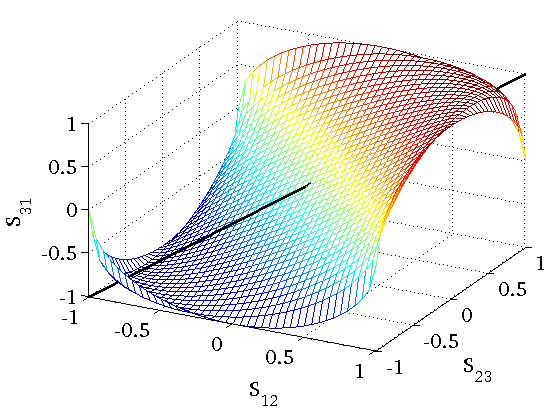
\includegraphics[width=8cm, angle=0]{cycle3b.png}
\caption{\label{fig:cycle3}
Geometric solution of the simplest cyclic network with
3 nodes with $P_j=0$ and three links with equal
strength $K$.
The black line is the solution space of the dynamical 
codition (\ref{eqn:3cycle-dc}) and the surface is the
relevant branch of the solution space of the geometrical
condition (\ref{eqn:3cycle-gc}). One finds three intersections 
corresponding to three stationary states.
}
\end{figure}

\subsection{Frustration induces discreteness.} 

We now extend the above example to a single cycle with an
arbitarry number of $N$ nodes with  the same frequency 
$P=0$. All links have an equal strength $K$ as above.
The dynamic conditions for a stationary states are then given by
\bea
  && F_{j+1,j} = F_{j,j-1}  \equiv F \qquad \forall j  \\ 
  && |F| \le K.
\eea
 The geometric condition yields
\bea
   && N \mbox{arcsin}(F/K) = 0 \quad (\mbox{mod} 2 \pi) \nn  \\
   \Rightarrow && F = K \sin(2\pi n/N), \qquad  n \in \mathbb{Z}\ \\  
   \Rightarrow && \phi_{j+1} - \phi_j = \frac{n}{N} 2 \pi
\eea
This shows that the dynamic condition has a continuum of 
solutions while the geometric condition induces a 
quantization of the phase differences 
$\phi_{j+1} - \phi_j$. 

In total we find $N$ different stationary states of this kind
with $n = 0,\ldots,N-1$,
taking into account that the phases are only defined modulo
$2\pi$. To determine the dynamic stability of these states,
we write the phases as $\phi_j(t) = \phi_j^* + \xi_j(t)$, where 
the star denotes the steady state value. To leading oder, the 
equations of motion for the $\xi_j$ are then given by 
\bea
   \frac{d}{dt} \xi_j &=& K \cos(2\pi n/N) 
      \left( \xi_{j+1} + \xi_{j-1} - 2 \xi_j \right) \nn \\
     &=:& \sum_i J_{j,i} \xi_i
\eea
The eigenvalues of the Jacobian matrix $J$ are given
by
\be
     {\rm eig}(J) = -4 K \cos(2\pi n/N) \sin^2(\pi k/N),
        \; k = 1,\ldots,N. \nn
\ee
Therefore we find that all steady states with 
$n \in [0,N/4]$ or $n\in[3N/4,N]$ are linearly stable.
 

This example is very simple but shows two important results
of ours most clearly which hold in general.
First, the Kuramoto model (\ref{eqn:kuramoto})
and the power grid model (\ref{eqn:power}) allow for 
steady states with a persitent current around a cycle.
Interestingly, theses states are phase locked but not phase
ordered in the sense that the phase order parameter
\be
   r e^{i \psi} := \frac{1}{N} \sum_j e^{i \phi_j} 
   \label{eqn:deforder}
\ee
vanishes exactly.
Second, the geometric condition induces the 
\emph{discreteness} of the phase differences
although the dynamic condition allows for arbitrary
large cycle flows.

\subsection{Braess' paradox}
\label{sec:braess}

Here we introduce a special example which illustrates the
paradoxial efffects of geometric frustration most clearly.
We consider the oscillator network depicted in Fig.~\ref{fig:braess} (a)
consisting of $N=6$ nodes placed on a cyclic network.
In particular, we analyze what happens if the capacity
of the upper edge is increased from $K$ to 
$\tilde K = K + \kappa$. 


\begin{figure}[tb]
\centering
\includegraphics[width=3.5cm, angle=0]{braess3}
\includegraphics[width=4.5cm, angle=0]{braess_order2}
\caption{\label{fig:braess}
Geometric frustration induces Braess' paradox.
(a) Topology of the network under consideration.
(b) Stability phase diagram: Order parameter $r$ 
as a function of $K$ and $\kappa$. No steady state exists 
in the white region. 
An increase of the local capacity $\kappa$ 
can induce loss of the phase locked state.
If not, it leads to an increase of the order parameter 
$r$.
}
\end{figure}

The dynamic condition for this network reads
\be
   0 = P_j + ( K_{j+1,j} S_{j+1,j}  - K_{j,j-1} S_{j,j-1} ),
  \label{eqn:dc-braess}
\ee
and $|\Delta_{j,j+1}| \le 1$, identifying node $j=7$ with $j=1$.
 For notational convenience,
we define the vector 
\be
   \vec S = (S_{6,1} ,S_{1,2}, \ldots, S_{5,6} ).
\ee
The solutions of the linear system of equations (\ref{eqn:dc-braess}) 
span a one-dimensional affine space parametrized by a real 
number $\epsilon$,
\be
   \vec S = \frac{P_0}{K} 
      \left( \vec S_a - \epsilon \, \vec S_b \right).
   \label{eqn:SaSb2}
\ee
The vector $\vec S_a = (1,1,0,-K/\tilde K,-1, 0)$ is the 
inhomogeneous solution of the linear system (\ref{eqn:dc-braess}), 
and the vector $\vec S_b = (2,1,1,2K/\tilde K,1,1)$is a homogeneous 
solution corresponding to a cycle flow.
Evaluating the condition $|S_{j,j+1}| \le 1$ yields
a necessary condition for the existstence of a stationary state
\be
     K \ge P_0.
\ee

For $\kappa = 0$ this condition is also sufficient for
the existence of a stationary state. If the capacity of the
upper link increases, $\kappa > 0$, geometric frustration
inhibits phase locking. A solution of the dynamical conditions
always  exists for   $K \ge P_0$, but this can become 
incompatible with the geometrix condtion as illustrated 
in the stability diagram  in Figure \ref{fig:braess} (b). No steady
state exists in the white region of parameter space. 
In the remaining region, we have plotted the Kuramoto phase 
order parameter (\ref{eqn:deforder})
in a color color.
One clearly observes that the unstable region \emph{increases} 
with $\kappa$. This leads to the paradoxial effect that
an increase of local transmission capacity reduces
the ability of the network to support a phase locked 
state. This behavior can also be seen as an example of 
Braess' paradox which has been first predicted for traffic 
network \cite{Brae68,12braess}.
 

\section{Conclusion}
Let Marc write this.




% --- Literatur -------------------------------------------------------------------

%\bibliography{networks,power,publwi}
\bibliography{epjst1}
\bibliographystyle{apsrev}




\end{document}
